\documentclass[justified, 11pt]{scrartcl}

% packages {
    \usepackage{amsmath, amsfonts, amsthm} 
    \usepackage{listings}
    \usepackage{inconsolata}
    \usepackage{graphicx}
    \usepackage{booktabs}
    \usepackage{enumitem}
    \usepackage{scrlayer-scrpage}
    \usepackage{sectsty}
    \usepackage{geometry} % Required for adjusting page dimensions and margins
    \usepackage[portuguese]{babel}
    \usepackage{booktabs}
    \usepackage{longtable}
    \usepackage{array}
    \usepackage{multirow}
    \usepackage{wrapfig}
    \usepackage{float}
    \usepackage{colortbl}
    \usepackage{pdflscape}
    \usepackage{tabu}
    \usepackage{threeparttable}
    \usepackage{threeparttablex}
    \usepackage[normalem]{ulem}
    \usepackage{makecell}
    \usepackage{xcolor}
    \usepackage{comment}
    \usepackage{lipsum}
    \usepackage{tabulary}
    \usepackage{tabularx}
    \usepackage{hyperref}
    \usepackage{cite}
    \usepackage{times}
    % \usepackage{showframe}
    \usepackage{fontspec}
    \usepackage{parskip}
    \usepackage[defaultsans,oldstyle,scale=0.95]{opensans}
    \usepackage[lining]{ebgaramond}
    \usepackage{textcomp}
    \usepackage{siunitx}
    \usepackage[tableposition=above]{caption}
    \usepackage{booktabs}
    \usepackage{tabulary}
% }


\sectionfont{\vspace{6pt}\scshape} % \section{} styling
\subsectionfont{\bfseries} % \subsection{} styling
\subsubsectionfont{\itshape} % \subsubsection{} styling
\paragraphfont{\scshape} % \paragraph{} styling

\ohead*{} % Right header
\ihead*{} % Left header
\chead*{} % Centre header

\ofoot*{} % Right footer
\ifoot*{} % Left footer
\cfoot*{\pagemark} % Centre footer

\geometry{
	paper=a4paper, % Paper size, change to letterpaper for US letter size
	top=2.5cm, % Top margin
	bottom=3cm, % Bottom margin
	left=3cm, % Left margin
	right=3cm, % Right margin
	headheight=0.75cm, % Header height
	footskip=1.5cm, % Space from the bottom margin to the baseline of the footer
	headsep=0.75cm, % Space from the top margin to the baseline of the header
	%showframe, % Uncomment to show how the type block is set on the page
}

\graphicspath{ {./figs/} }

\setlength{\parindent}{2em}

\setcounter{secnumdepth}{0}

\addfontfeatures{Numbers={Lining}}

\newcommand{\email}[1]{\small{\href{mailto:#1}{#1}}}
\makeatletter
\NewDocumentCommand{\mynote}{+O{}+m}{%
  \begingroup
  \tcbset{%
    noteshift/.store in=\mynote@shift,
    noteshift=1.5cm
  }
  \begin{tcolorbox}[nobeforeafter,
    enhanced,
    sharp corners,
    toprule=1pt,
    bottomrule=1pt,
    leftrule=0pt,
    rightrule=0pt,
    colback=yellow!20,
    #1,
    left skip=\mynote@shift,
    right skip=\mynote@shift,
    overlay={\node[right] (mynotenode) at ([xshift=-\mynote@shift]frame.west) {\textbf{Note:}} ;},
    ]
    #2
  \end{tcolorbox}
  \endgroup
  }
\makeatother

\title{	
	\normalfont\normalsize
	\textsc{ISCTE-IUL \\ Licenciatura em Ciência de Dados}\\
	\vspace{20pt} 
	\rule{\linewidth}{0.5pt}\\
	\vspace{20pt}
	{\huge Previsão do desempenho de estudantes ao jogar}\\ 
  \vspace{16pt} 
  {\large Trabalho realizado no âmbito da Unidade Curricular Processamento de Big Data do 2º ano em 2022/2023 da Licenciatura em Ciência de Dados}\\
	\vspace{12pt}
	\rule{\linewidth}{2pt}\\
	\vspace{20pt} 
}
\author{
  André Plancha, 105289 \\
  \email{Andre\_Plancha@iscte-iul.pt}\\
  Allan Kardec Rodrigues, 103380 \\
  \email{aksrs@iscte-iul.pt} \\
  \vspace{30pt}
}
\date{9 Abril 2023 \\ Versão 1.0.0}

\begin{document}
  \thispagestyle{empty}
  \maketitle
  \pagebreak
  \section{Introdução}
  \textbf{Jo Wilder and the Capitol Case} é um jogo educacional sobre a história de Wisconsin, direcionado a crianças com idades entre os 8 e os 12 anos. O jogo de aventura e investigação segue a história de Jo Wilder, que descobre histórias sobre artefactos do passado do estado, investigando objetos, e encontrando pessoas. O jogo pode ser jogado no site oficial do PBD Wisconsin Education\footnote{\url{pbswisconsineducation.org/jowilder/play-the-game/}}. Esta competição está a ser promovida pela plataforma kaggle\footnote{\url{https://www.kaggle.com/competitions/predict-student-performance-from-game-play}}.

  \begin{figure}[h]
    \centering
    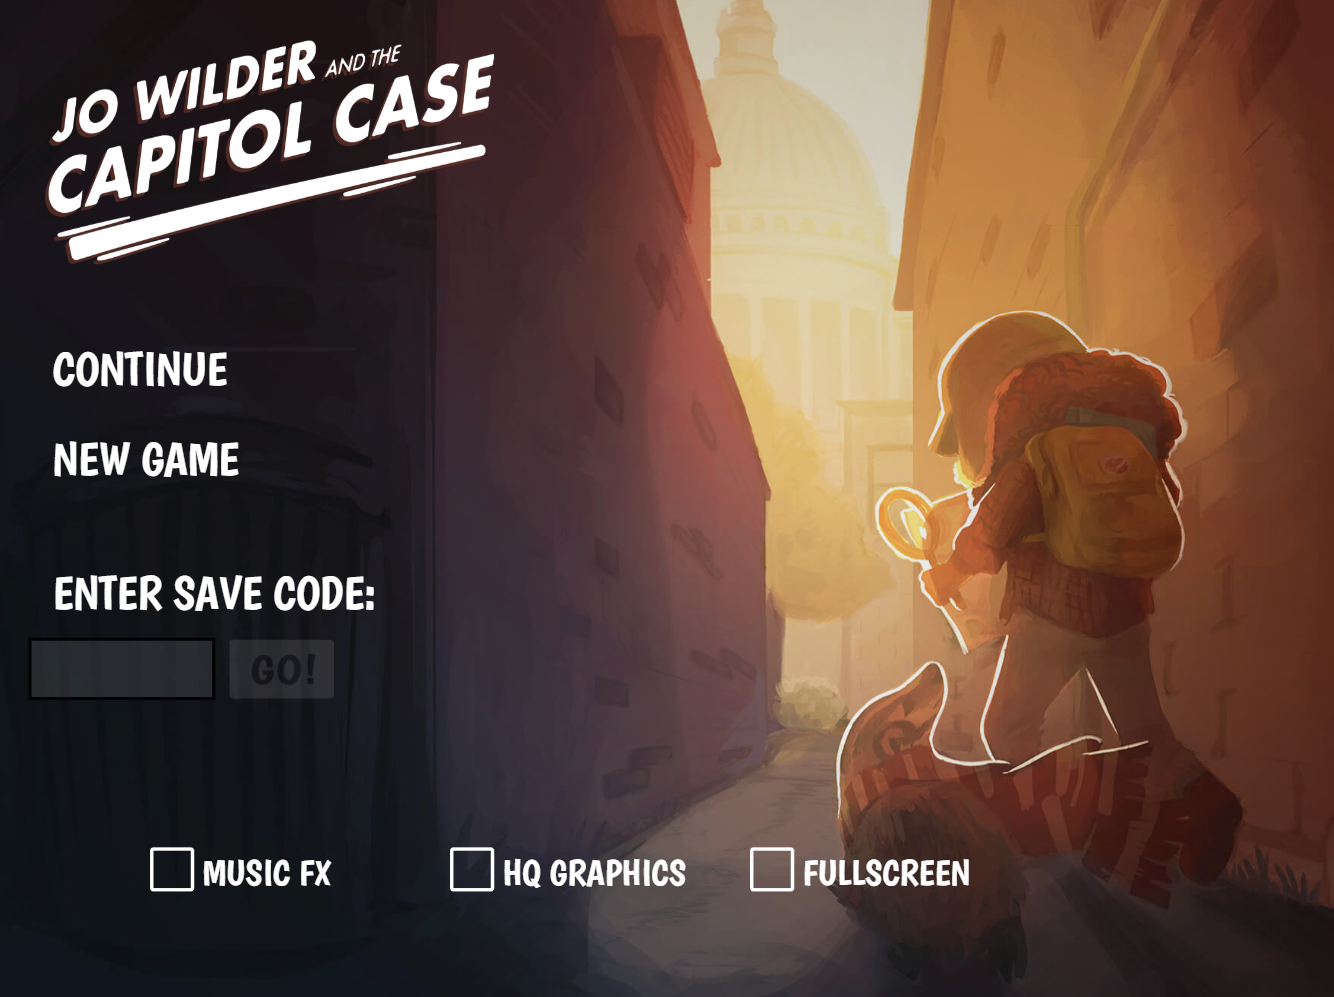
\includegraphics[width=0.8\linewidth]{jo_wilder.png}
    \caption{Imagem do menu principal}
    \label{fig:jo_wilder}
  \end{figure}

  Este projeto tem como objetivo prever como os jogadores vão responder às 18 questões que o jogo apresenta, baseado na sua atividade durante o tal, implementando uma solução computacional para estudo e análise de dados de grande dimensão. Para isso, vamos usar Apache Spark\texttrademark e \textit{PySpark} para processar os dados e a biblioteca \textit{MLlib} para a criação de um modelo de aprendizagem supervisionada.

  \section{Análise exploratória dos dados}
  
  A competição disponibiliza um conjunto de ficheiros de dados, nos quais 2 são de interesse: \texttt{train.csv} e \texttt{train\_labels.csv}, elas tendo as variáveis de interesse e as respetivas respostas, respetivamente. \texttt{train.csv} contém as seguintes colunas\footnote{Mais informações sobre cada coluna está no site da competição, e no EDA em anexo}, entre outras:
  \begin{itemize}
    \item \texttt{session\_id}: Identificador da sessão do evento.
    \item \texttt{index}: Índice do evento na sessão.
    \item \texttt{elapsed\_time}: Tempo decorrido desde o início da sessão em \si{\milli\second}.
    \item \texttt{event\_name}: Tipo do evento.
    \item \texttt{name}: Específicos do tipo de evento.
    \item \texttt{hover\_duration}: O tempo de permanência do cursor sobre um objeto, em \si{\milli\second}, se aplicável.
    \item \texttt{text}: O diálogo/monólogo que o jogador viu no evento, se aplicável
    \item \texttt{fqid}: O identificador único do evento.
    \item \texttt{fullscreen}: Se o jogador está em modo de ecrã inteiro.
    \item \texttt{hq}: Se o jogo está em alta qualidade.
    \item \texttt{music}: Se a música do jogo está ligada.
    \item \texttt{level\_group}: O grupo de níveis a que o evento pertence.
  \end{itemize}
  ; e \texttt{train\_labels.csv} contém as seguintes colunas:
  \begin{itemize}
    \item \texttt{session\_id}: Identificador da sessão do evento, em conjunto da pergunta que se pretende responder.
    \item \texttt{correct}: Se a pergunta está correta ou não.
  \end{itemize}

  Perante as colunas, como há uma incompatibilidade entre perguntas e respostas, nós decidimos criar uma tabela com cada sessão, características de tal (recursos) e as suas respostas, de forma usar classificação para prever as respostas.

  Para criar estes recursos, foi necessário de uma análise dos tipos de eventos disponíveis. Uma análise mais aprofundada encontra-se em anexo, mas para resumir, os eventos estão dividídos em 3 categorias: Exploração, exposição e revisao. Exploração são os eventos onde a personagem se move, interage com objetos opcionais, tenta entrar em zonas ainda não acedidadas, etc... Exposição são os eventos onde a personagem interage com personagens, interage com objetivos principais, e é onde se encontra o que o utilizador aprende. Revisão são os eventos de quando o utilizador está perdido e portanto precisa de apoio de qual é o próximo passo.

  A única excepção a estes eventos é o evento \texttt{checkpoint}, representando quando o utilizador começa a responder às perguntas (os eventos das respostas às perguntas não se encontra na tabela). Há 3 zonas onde o utilizador responde às perguntas, e na base de dados as 3 zonas são divididas pelos \texttt{checkpoint}s, e cada zona está rotulada pelo seu \texttt{level\_group}.

  \subsection{Análise e limpeza}
  Nós usámos como base de limpeza a nossa análise, e a análise de erros de um utilizador do kaggle\footnote{\url{https://www.kaggle.com/code/abaojiang/eda-on-game-progress}}. Na \autoref{tab:problemas} encontra-se os problemas encontrados e as soluções que nós usámos para os resolver.
  \begin{table}[htb]
    \centering
    \caption{Resolução dos problemas}
    \label{tab:problemas}
    \setlength{\extrarowheight}{7pt}
    \begin{tabulary}{\textwidth}{ L L L L }
      \toprule
      Erros & Problemas & Solução & Notas \\
      \midrule
      Tempo recorrido recuáva no tempo & Cálculo de tempos entre eventos pode ficar inválido & Transformar em diferenças entre os tempos e tornar zero quando negativo & Máximo desta coluna continua afetado \\
      Saltos de \texttt{index} & O índice do evento não é sequencial & - & Suspeitamos que os eventos aconteceram na mesma, só não foram anotados\\
      Sessões com menos ou mais de 3 checkpoints & As sessões são inválidas e dificultam análise & Foram removidas essas sessões & \\
      Tempos de jogo demasiado elevados comparado com a maioria dos tempos & Dificulta o processo de aprendizagem & Tempos de jogo foram transformados e normalizados &
    \end{tabulary}
  \end{table}

  Algumas das limpezas foram úteis na criação dos recursos, enquanto que outras apenas limparam a base de dados. Nós não fizemos (nem registámos) algumas das limpezas, pois não seria benéfico para a criação dos recursos necessários.

  Algo importante a notar também é que os roteiros dos jogos são diferentes para cada utilizador, entre 4 roteiros diferentes: \textit{dry}, \textit{nohumor}, \textit{nosnark}, e \textit{normal}. Um exemplo pode ser encontrado na \autoref{fig:textDiffs}. A diferença entre roteiros é mínima na opinião dos autores, mas decidimos usar esta informação na mesma.
  \begin{figure}[H]
    \centering
    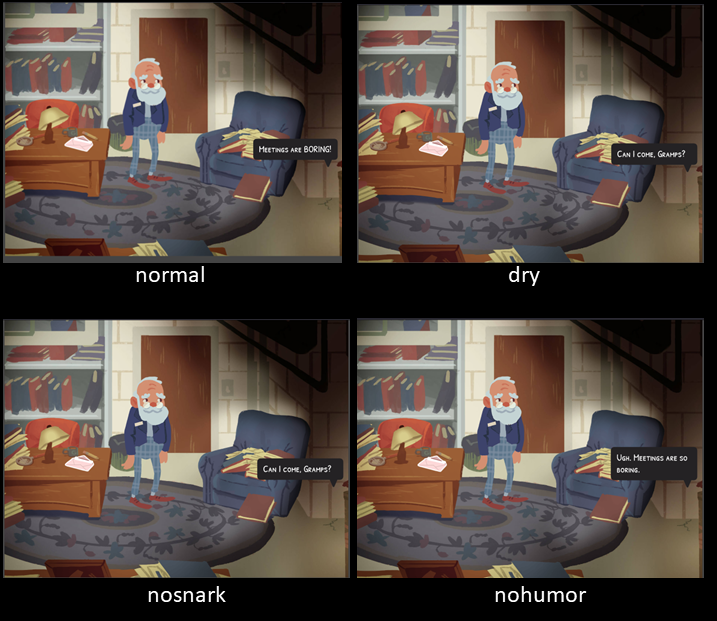
\includegraphics[width=0.8\linewidth]{text_differences.png}
    \caption{Diferenças entre roteiros}
    \label{fig:textDiffs}
  \end{figure}

  \subsection{Processo}
  O processo da implementação da solução computacional pode ser descrito como caótico, sendo que como os dados não vieram com uma estrutura clara, foi necessário uma representação dos dados adaptada previamente ao análise de relações entre os dados; ou seja a criação de recursos teóricos foi executada \textit{à priori}, e a análise de colineariadade e de relação foi feita \textit{ad hoc}. Por outras palavras, a análise de dados foi feita ao longo do processo de criação de recursos, e a criação destes foram feitos apenas com análises comportamentais potências invés de análises estatísticas. Ainda assim, a \autoref{fig:processo} pode ser visto o processo que foi seguido.

  \begin{figure}[H]
    \centering
    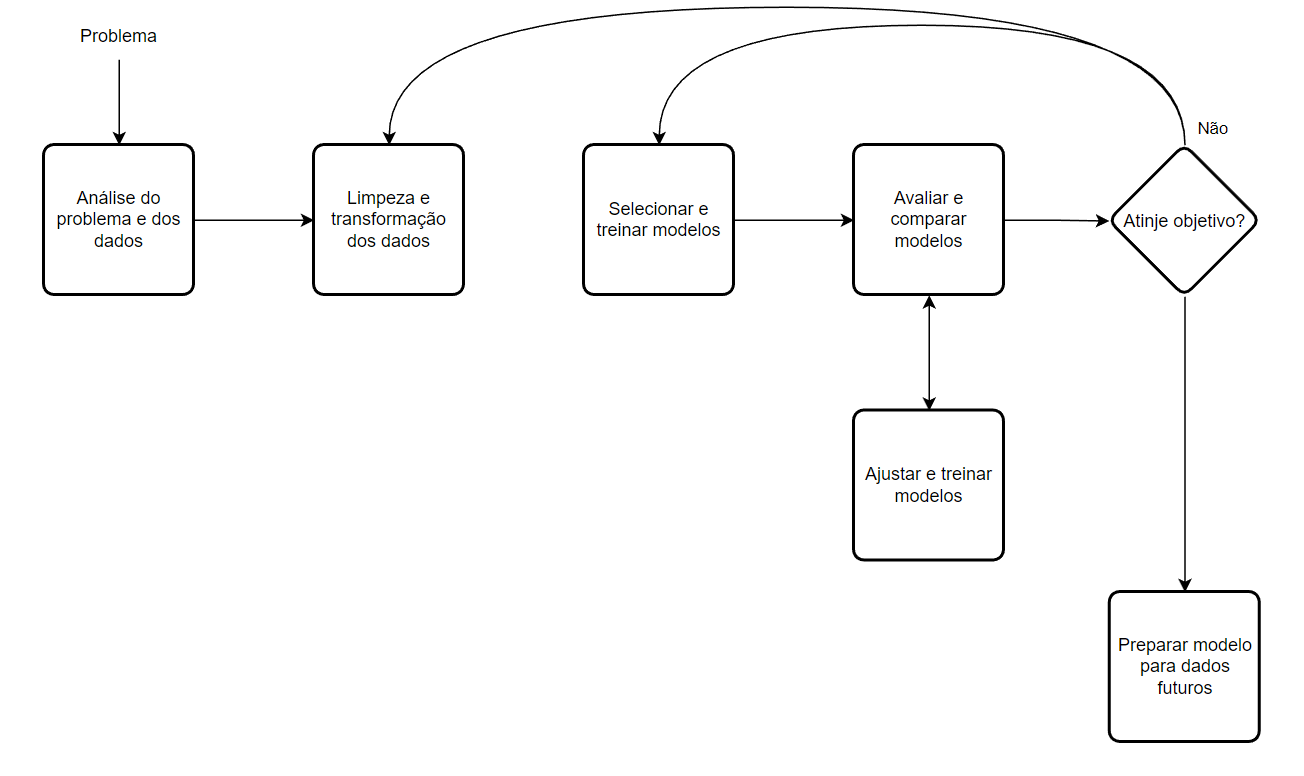
\includegraphics[width=0.8\linewidth]{processo.png}
    \caption{Processo}
    \label{fig:processo}
  \end{figure}
  
  \subsection{Recursos}
  As features que nós fizemos para cada sessão são entre as seguintes:
  \begin{itemize}
    \item O index máximo, que indica o número de eventos de cada sessão;
    \item Se a sessão esteve em tela cheia;
    \item Se a sessão estava em alta qualidade;
    \item Se a sessão tinha música ligada;
    \item Quantos objetivos opcionais a sessão interagiu com;
    \item Quantas salas inacessíveis a sessão tentou entrar em;
    \item Quantas vezes a sessão reviu o objetivo;
    \item Tempo médio de leitura do diálogo;
    \item Tempo médio por movimento do jogador;
    \item Tipo de roteiro.
  \end{itemize}

  Os promenores de como foram criadas encontram-se em anexo.

  \subsection{Exploração}
  Devido à natureza dos nossos dados a exploração não foi executada de uma forma tradicional, sendo que as análises menos teóricas foram feitas após a criação de cada recurso. De qualquer forma, estas encontram-se em anexo. Ainda assim, anotaremos aqui a análise de probabilidades das respostas.

  \begin{figure}[H]
    \centering
    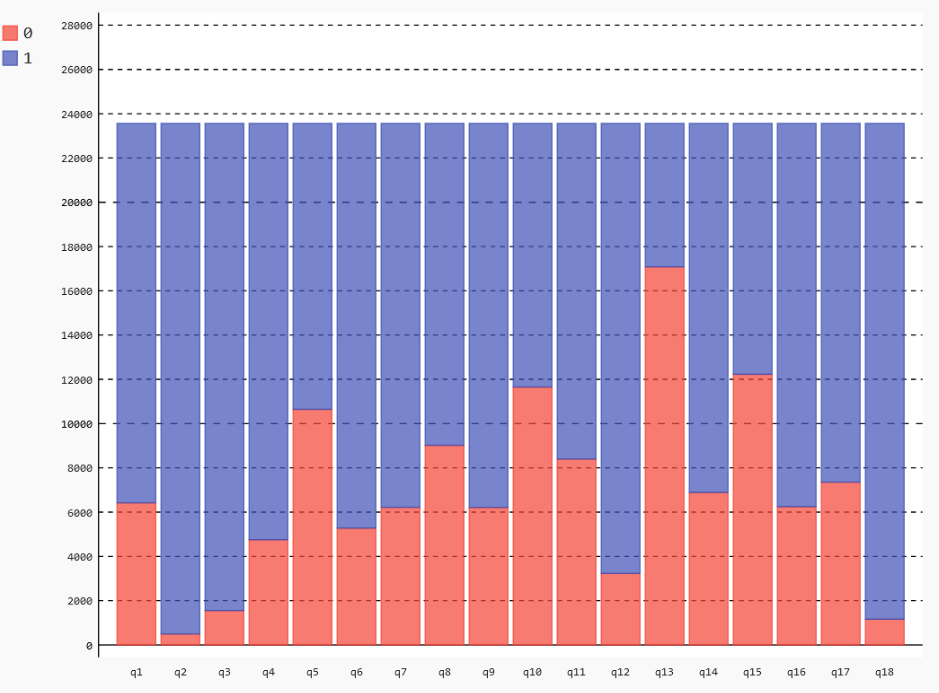
\includegraphics[width=0.7\linewidth]{probs.png}
    \caption{Probabilidades das respostas}
    \label{fig:probs}
  \end{figure}

  Como se pode opbservar na \autoref{fig:probs}, algumas respostas são muito prováveis de acertar, e poucas são mais prováveis de errar. Notamos que há um acréscimo de perguntas erradas nas questões 5 e 13, sendo que essas são as primeiras do grupo. Ainda assi, não parece haver um padrão claro.
  \section{Modelação}
  Como processo de modelação, nós usámos aprendizagem supervisionada de classificação multi-rótulo, usando como rótulos cada pergunta certa, ou seja, cada sessão podia ter entre 0 e 18 rótulos. Nós considerámos várias opções de classificação, mas decidimos que a melhor forma para o nosso projeto foi com uma transformação para um problema de classificação binária, usando o método de \textit{binary relevance}.
  
  De forma simplificada, para cada rótulo, um modelo binário é treinado, independente dos outros rótulo; se 1 o rótulo é incluido, se 0 não. Esta estratégia fazia sentido, sendo que os nossos rótulo já são binários, o que facilita a modelação, e como temos uma grande quantidade de rótulos, outras estratégias (como \textit{Label Powerset}) não faziam tanto sentido. Ainda assim, pode haver outros métodos mais adequados, como por exemplo \textit{Classifier Chains}, sendo que não deve haver uma indepenência de rótulos.

  Para a análise dos nossos modelos, usámos métricas de classificação multi-rótulo, como o \textit{subset accuracy}, \textit{hamming loss}, e \textit{micro-F1}. Usámos também a métrica de avaliação \textit{F1}, estrapulada e adaptada.

  \textit{Subset accuracy} é uma métrica que mede a percentagem de resultados que todos os rótulos estão certos. Previmos que esta métrica não seira muito útil, sendo que 18 rótulos corretos é muito difícil do nosso modelo conseguir, especialmente com o método de \textit{binary relevance}.
  $$
  \uparrow \mathnormal{subset\text{-}accuracy} = \frac{1}{|Y|} \sum_{i=1}^{|Y|}  \left[ 
    \hat{Y}_i = Y_i
    \right] 
  $$
  \textit{Hamming loss} é uma métrica que mede a percentagem de rótulos que estão errados. Sendo que este mede de forma mais individual, esta métrica é mais útil e direta.
  $$
  \downarrow \mathnormal{hamming\text{-}loss} = \frac{1}{|Y|\cdot|L|} \sum_{i=1}^{|Y|} \sum_{l=1}^{|L|} \left[ 
    \hat{Y}_{i,l} \neq Y_{i,l}
    \right]
  $$
  \textit{Micro-F1} é uma métrica que mede a percentagem de rótulos que estão certos, mas penaliza mais os rótulos que estão errados. Esta métrica é útil mais útil para comparar modelos, em vez de ser útil para avaliar o modelo individualmente.

  $$
  \uparrow \mathnormal{micro\text{-}}F_1 = \frac{2 TP}{2TP + FP + FN}
  $$
  \textit{F1} é uma métrica usada para avaliar modelos de classificação binária, e é uma média ponderada entre a precisão e a revocação. A nossa métrica adaptada faz a média dos vários F1 scores de cada modelo que compoz o algoritmo. Esta métrica é também útil para comparar modelos, pois dá igual importância a cada modelo, enquanto que a mética anterior tem em conta a quantidade de rótulos que cada $X$ tem, no nosso caso isso equivaler às respostas certas, o que pode induzir em erro a métrica.

  $$
  \uparrow F_1 = \frac{2}{|Y|} \sum_{i=1}^{|Y|} 
    \frac{\left| Y_i \cap \hat{Y}_i \right|}{| Y_i | + | \hat{Y}_i |}
  $$

  
  Nós começámos por treinar 4 modelos, de forma a compará-los e decidir que método usar, sendo eles regressão logística, máquna de vetores de suporte linear, árvore de decição e \textit{random forest}, todos eles com o método de \textit{binary relevance}. Os promenores do executado e dos parametros estão em anexo. Os resultados podem ser observados na \autoref{tab:results}.
  %{'subSetAcc': 0.02224242100197829, 'hammingLoss': 0.2477410041169866, 'microF1Measure': 0.8411937081458605, 'regularF1': 0.8239368537828183}
  %{'subSetAcc': 0.022937496658290115, 'hammingLoss': 0.25165897330790665, 'microF1Measure': 0.8423530374979532, 'regularF1': 0.8284907895850899}
  %{'subSetAcc': 0.02368603967277977, 'hammingLoss': 0.24395967373029878, 'microF1Measure': 0.8429258291672563, 'regularF1': 0.8268147783725285}
  %{'subSetAcc': 0.023204833449179275, 'hammingLoss': 0.24422106970361263, 'microF1Measure': 0.844419634409416, 'regularF1': 0.8295224110560213}
  \begin{table}[H]
    \centering
    \caption{Resultados dos primeiros modelos}
    \setlength{\extrarowheight}{0pt}
    \begin{tabulary}{\textwidth}{ L|r r r r }
      %\toprule
      Modelo & \myalign{l}{Subset accuracy $\uparrow$} & \myalign{l}{Hamming loss $\downarrow$} & \myalign{l}{Micro-F1 $\uparrow$} & \myalign{l}{F1 $\uparrow$} \\ \hline
      Regressão Logística & $0.0222$ & $0.2477$ & $0.8412$ & $0.8239$ \\
      Máquina de Vetores de Suporte Linear & $0.0229$ & $0.2517$ & $0.8424$ & $0.8285$ \\
      Árvore de Decisão & $\boldsymbol{0.0237}$ & $\boldsymbol{0.2440}$ & $0.8429$ & $0.8268$ \\
      Random Forest & $0.0232$ & $0.2442$ & $\boldsymbol{0.8444}$ & $\boldsymbol{0.8295}$ \\
    \end{tabulary}
    \label{tab:results}
  \end{table}
  
  Como se pode observar, estes modelos não mostram muita diferença nos resultados, mesmo que a árvore de decisão tenha um resultado melhor nas métricas individuais, e o Random Forest tenha obtido um melhor resultado nas métricas de comparação. Decidimos tentar melhorá-los, tirando proveito destes resultados. Logo, treiná-mos mais 4 modelos \textit{Random Forest}, com parâmetros diferentes, especicamente na estratégia de divisão em cada nó. Mais promenores sobre este processo estão na documentação da classe \textit{RandomForest} \footnote{\url{https://spark.apache.org/docs/latest/api/python/reference/api/pyspark.mllib.tree.RandomForest.html}}. Os resultados pdoem ser observados na \autoref{tab:results2}.
  %{'subSetAcc': 0.024701919478158585, 'hammingLoss': 0.24197544066014365, 'microF1Measure': 0.84481655046291, 'regularF1': 0.8288088968104772}
  %{'subSetAcc': 0.023204833449179275, 'hammingLoss': 0.24422106970361263, 'microF1Measure': 0.844419634409416, 'regularF1': 0.8295224110560213}
  %{'subSetAcc': 0.023204833449179275, 'hammingLoss': 0.24422106970361263, 'microF1Measure': 0.844419634409416, 'regularF1': 0.8295224110560213}
  %{'subSetAcc': 0.02422071325455809, 'hammingLoss': 0.24346658587154765, 'microF1Measure': 0.8448010118874048, 'regularF1': 0.8297927984968329}
  \begin{table}[H]
    \centering
    \caption{Resultados dos segundos modelos}
    \setlength{\extrarowheight}{0pt}
    \begin{tabulary}{\textwidth}{ L|r r r r }
      %\toprule
      Modelo & \myalign{l}{Subset accuracy $\uparrow$} & \myalign{l}{Hamming loss $\downarrow$} & \myalign{l}{Micro-F1 $\uparrow$} & \myalign{l}{F1 $\uparrow$} \\ \hline
      RF - all & $\boldsymbol{0.0247}$ & $\boldsymbol{0.2420}$ & $\boldsymbol{0.84481}$ & $0.8288$ \\
      RF - sqrt/log2 & $0.0232$ & $0.2442$ & $0.84442$ & $0.8295$ \\
      RF - onethird & $0.0242$ & $0.2435$ & $0.84480$ & $\boldsymbol{0.8298}$ \\
    \end{tabulary}
    \label{tab:results2}
  \end{table}

  Como se pode observar, as diferenças são minúsculas o suficiente que dificilmente se considera um melhor que o outro. Ainda assim, o modelo \textit{RF} com estratégia \textit{all} tem um resultado individual melhor, e \textit{RF} com estratégia \textit{onethird} tem um resultado de comparação melhor. Como os resultados não parecem melhorar tanto assim, e como temos já bons resultados com os modelos apresentados, decidimos não continuar a modelar.

  Pela a análise das matrizes de confusão (em anexo), podemos observar muitas das perguntas sem positivos ou negativos. Isto é devido à própria amostra que tinhamos acesso não ter muitas respostas positivas ou negativas para as perguntas em quastão. Isto devia ter sido verificado antes de começar, e devia ter-se adaptado a forma de divisão em conjunto de treino ou teste, ou devia ter-se usado validação cruzada.

  Para melhorar o resultado, além do referido podia-se também ter-se melhorado a limpeza dos dados, sendo que há muitas sessões com valores inválidos, que podiam ter sido tratados e/ou as sessões removidas do conjunto de treino.

  \begin{figure}[H]
    \centering
    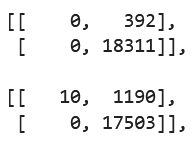
\includegraphics[width=0.2\textwidth]{confusion.png}
    \caption{Exemplos de matrizes de confusão resultadas por rótulo}
    \label{fig:confusion_matrix}
  \end{figure}

  \subsection{Tempo de execução}
  De forma a comparar as ferramentas que tinha-mos disponíveis, decidimos medir o tempo de execução dos 4 primeiro modelos apresentados, uma primeira vez com o ambiente local, outra com 5 clusters da Amazon EMR (AWS) . O ambiente local usado é composto por um AMD Ryzen 7 5800X com 8 cores (16 Threads). Os resultados podem ser observados na  \autoref{tab:time}.
  \begin{table}[H]
    \centering
    \caption{Tempo de execução}
    \setlength{\extrarowheight}{0pt}
    \begin{tabulary}{\textwidth}{ L|r r r }
      %\toprule
      Modelo & \myalign{l}{Local (\si{\milli\second})} & \myalign{l}{AWS (\si{\milli\second})}  & \myalign{l}{Diferença (\%)} \\ \hline
      Regressão Logística & $16.743$ & $51.014$ & $304.7$\\
      SVM & $41.470$ & $112.787$ & $272.0$  \\
      Árvore de Decisão & $9.962$ & $35.154$ & $352.9$\\
      Random Forest & $15.247$ & $46.656$ & $306.0$\\
    \end{tabulary}
    \label{tab:time}
  \end{table}

  Como podemos observar, o uso do AWS no nosso caso piorou o tempo de execução. No entanto, não descartamos a ferramenta para ambientes pessoais menos potentes, e a sua utilidade também pode ser observada para outros casos específicos. Também não tiramos proveito de todas as funcionalidades do serviço, portanto estes números podem não estar optimizados.
\end{document}

